\documentclass[11pt,leqno]{article}
\usepackage[utf8]{inputenc}
\usepackage{tikz} 
\usepackage{array}
\usepackage{graphicx}
\graphicspath{ {./images/} }
\title{Tema practica}
\author{Socoteală Andrei Alin, Adăscăliței Robert Marian}
\date{Jan 2024}
\begin{document}
	\maketitle
	\vspace{5mm}
{\large \underline{ Intelegerea setului de date} }
	\\\\
	{\normalsize 
		Setul de date contine 4 foldere (lemm, bare, lemm\_stop si stop), iar fiecare folder contine alte 10 foldere care contin email-uri (part1-part10). Mesajele de tip spam contin in titlu cuvantul "spm". Pentru rezolvare, am folosit folderul bare, iar aici am utilizat primele 9 foldere pentru antrenare, iar folderul 10 pentru testare. Pentru procesarea datelor, am folosit o metoda simpla: am utilizat un dictionar care contine contentul email-ului si eticheta "spam" (daca mesajul este spam) sau eticheta "regular" (daca mesajul nu este spam). Clasificarea in email spam sau email regular se face dupa numele fisierului (daca contine "spm" este spam, altfel regular). Functia care clasifica email-urile poate fi vazuta mai jos. \\
		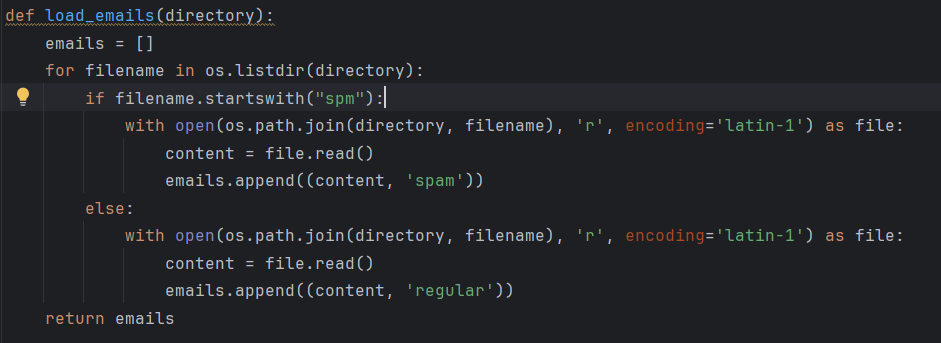
\includegraphics[scale=0.8]{load}
		\\
		In continuare, pentru partea de antrenare, se extrage fiecare cuvant din fiecare email si creste count-ul (count-ul pentru spam daca a fost gasit intr-un email spam sau count-ul pentru regular daca a fost gasit intr-un email regular). In final, dupa faza de antrenare, vom avea doua dictionare, unul pentru cuvinte spam, unul pentru cuvinte regular care vor contine cuvinte si respectiv count-ul lor. Mai jos, functia tokenize si functia de antrenare:\\
		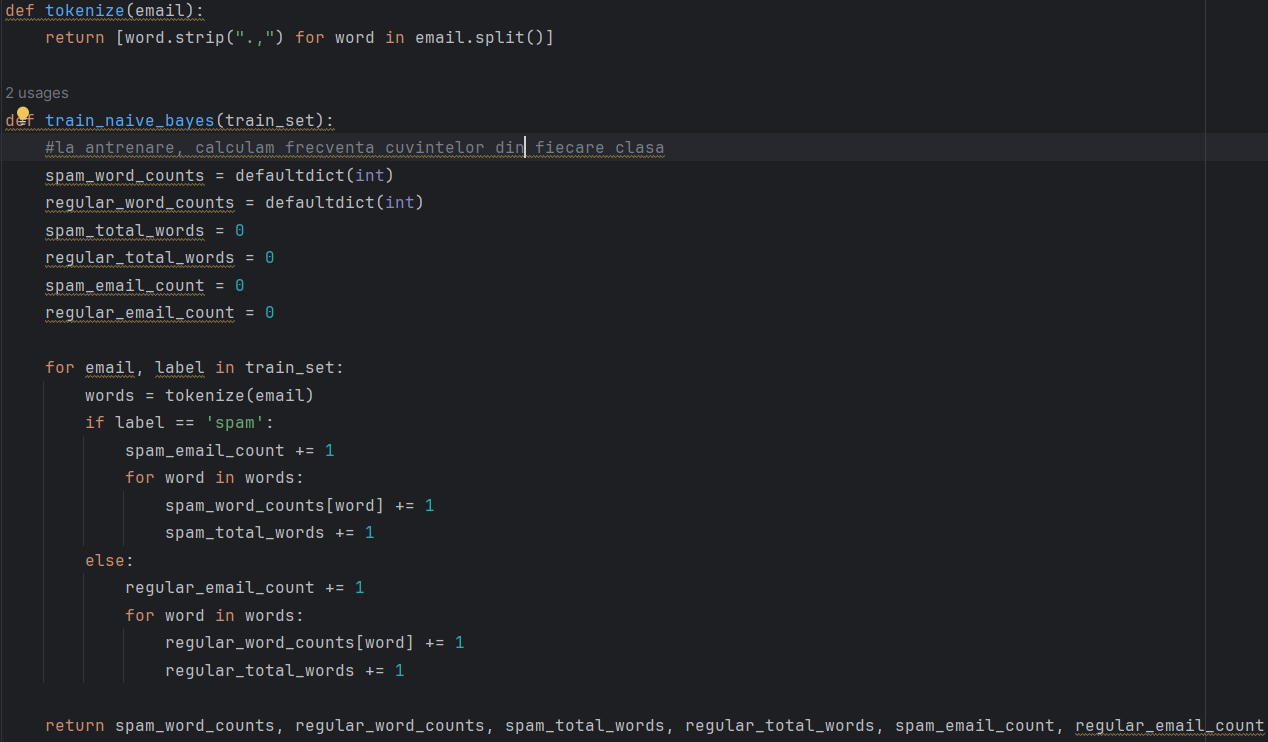
\includegraphics[scale=0.6]{train}
	}
	\\\\
	{\large \underline{Alegerea algoritmului} }
	\\\\
	{\normalsize 
		Pentru problema clasificarii email-urilor spam din setul de date Ling-Spam am ales algoritmul Naive Bayes, performantele acestuia pot fi vazute, in imaginea ce urmeaza, atat grafic cat si text:\\
		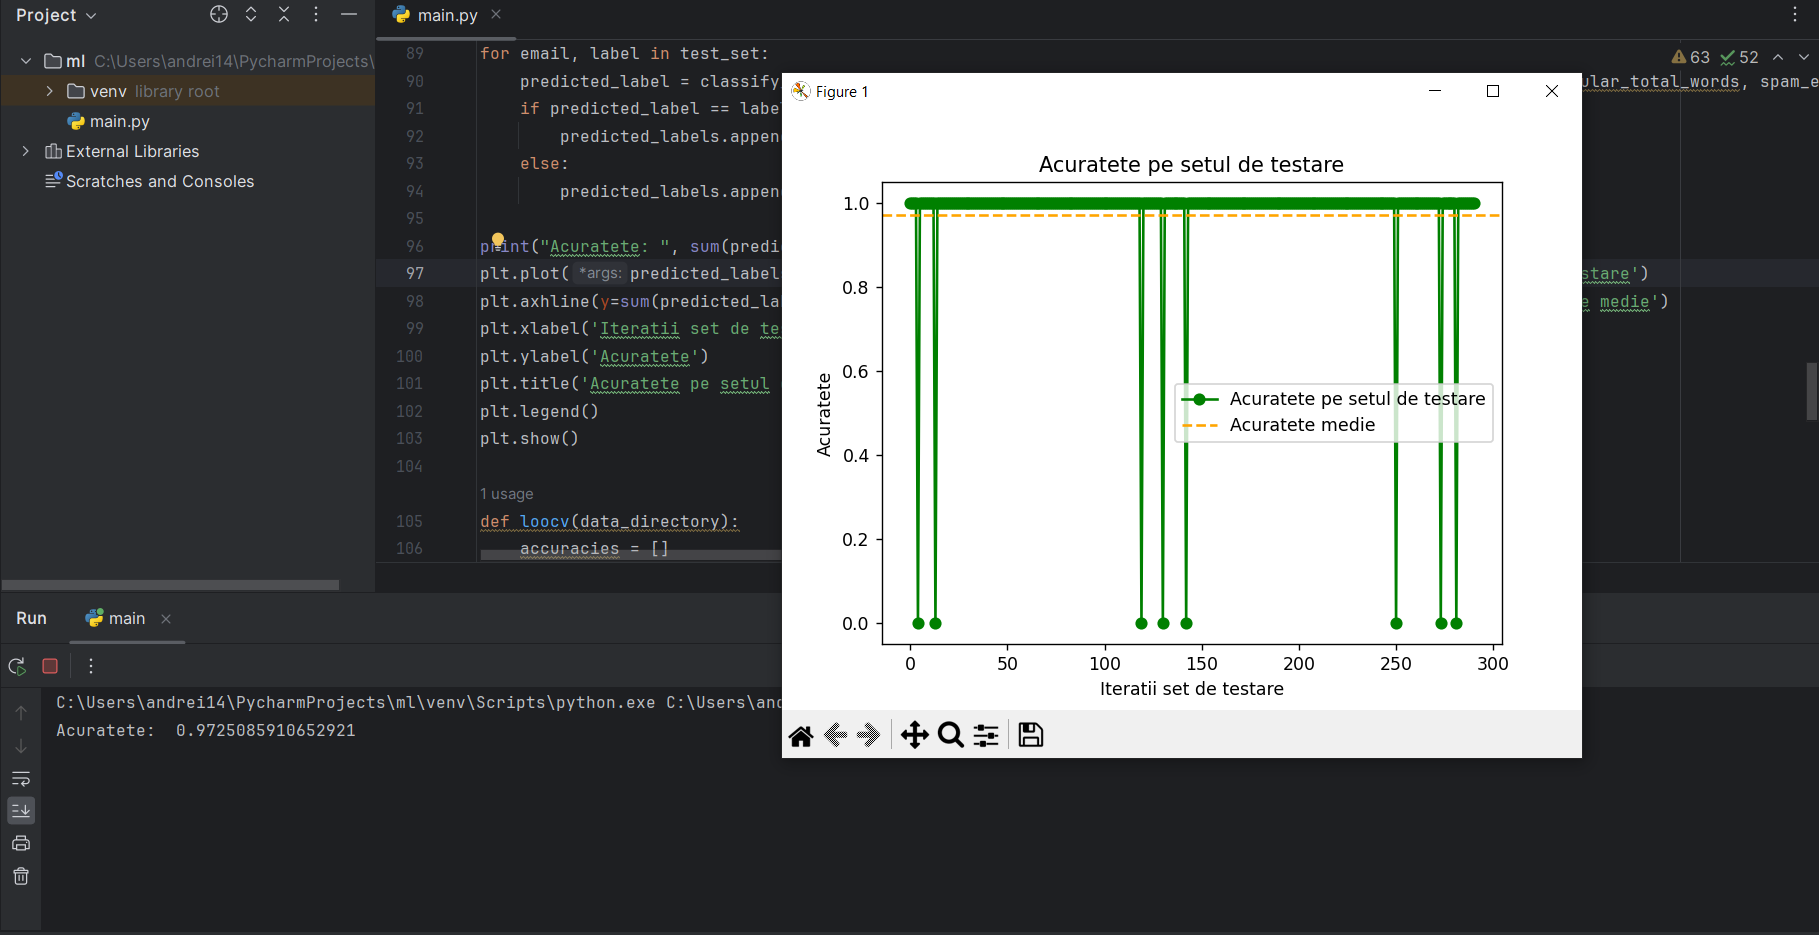
\includegraphics[scale=0.5]{acuratetetestare}
		\\\\
			\textit{Justificare teoretica:}\\
			Naive Bayes se bazeaza pe teorema lui Bayes si are presupozitia ca toate caracteristicile sunt independente intre ele data fiind clasa. In contextul clasificarii email-urilor spam, aceasta abordare simplificata se potriveste bine, deoarece email-urile pot avea un numar mare de cuvinte si caractere, iar presupozitia de independenta poate facilita calculul probabilitatilor conditionate. De asemenea, Naive Bayes este eficient in gestionarea datelor rare si este rapid de antrenat, ceea ce îl face potrivit pentru seturi de date de dimensiuni mari, cum ar fi colectiile de email-uri.	Naive Bayes este, de asemenea, adesea folosit pentru clasificari bazate pe text (exact ca si in cazul email-urilor) \\
			Din acest motiv am ales Naive Bayes si nu, de exemplu ID3, unde, avand un set de date foarte complex, performanta putea fi afectata (de exemplu, din cauza overfitting-ului). 
		\\\\
		\textit{Justificare practica:}\\
		Mai sus am aratat acuratetea pe setul de testare pentru algoritmul Bayes Naiv, care este una de aproximativ 97\%
		, o acurtatete mult mai buna decat o acuratete pentru datul cu banul sau alegerea aceleiasi clase intotdeauna (daca alegeam intotdeauna clasa regular, am fi avut acuratete de 83\%, deoarece in bare-part10 sunt 242 mesaje regular si 49 mesaje spam).\\
		In plus, am testat acelasi set de date si pentru un clasificator de tipul Adaboost, folosind 5 iteratii, acuratetea in acest caz fiind de 82\%, adica aproximativ cat cea de la alegerea clasei regular intotdeauna. \\\\
		ACURATETE ADABOOST 5 ITERATII\\
		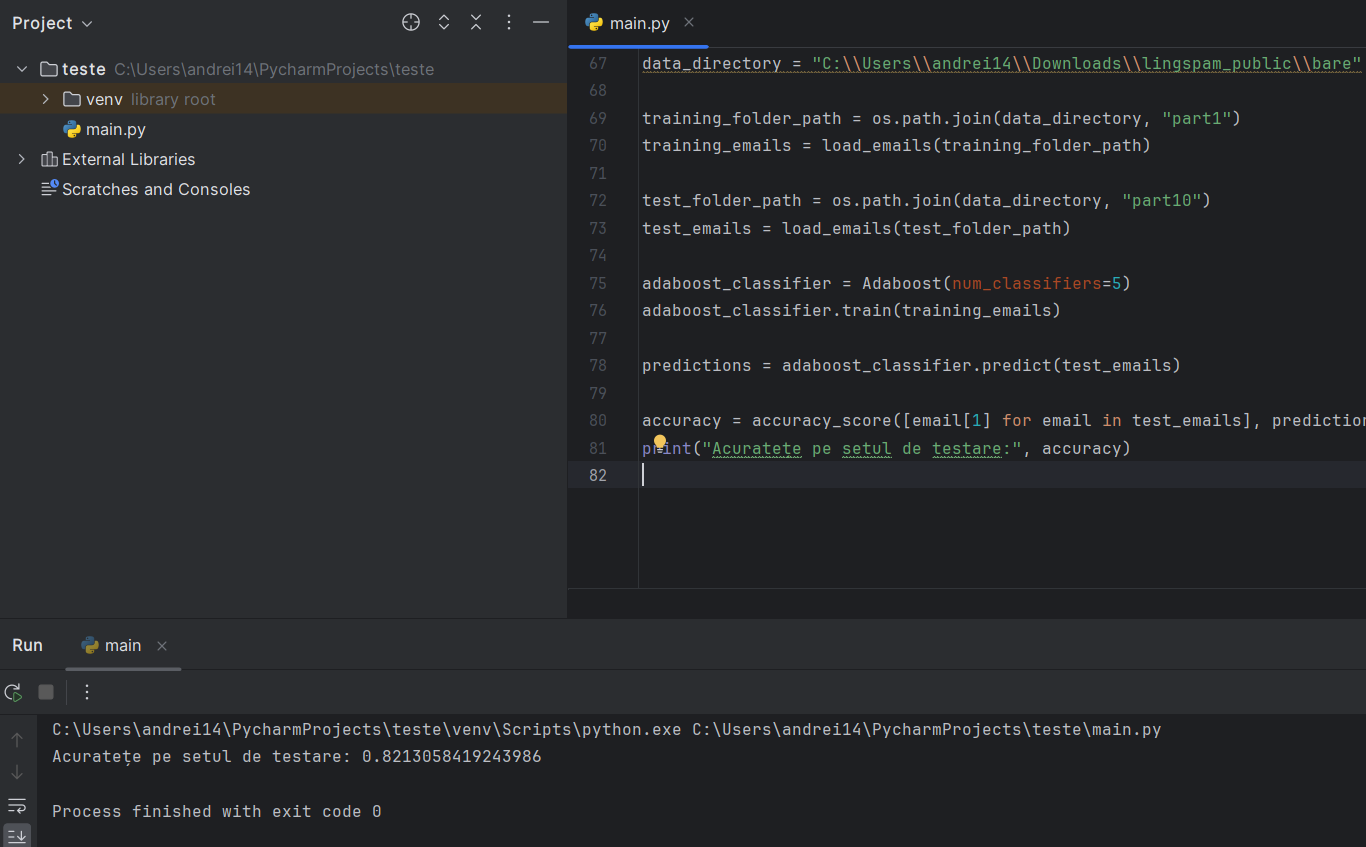
\includegraphics[scale=0.6]{adaboost} \\\\
		Pentru un clasificator de tipul Adaboost dar doar cu 2 iteratii, am obtinut o acuratete de 92\%, mult mai buna decat cea anterioara, dar totusi sub cea obtinuta cu Naive Bayes.\\\\\\\\\\\\
		ACURATETE ADABOOST 2 ITERATII\\
		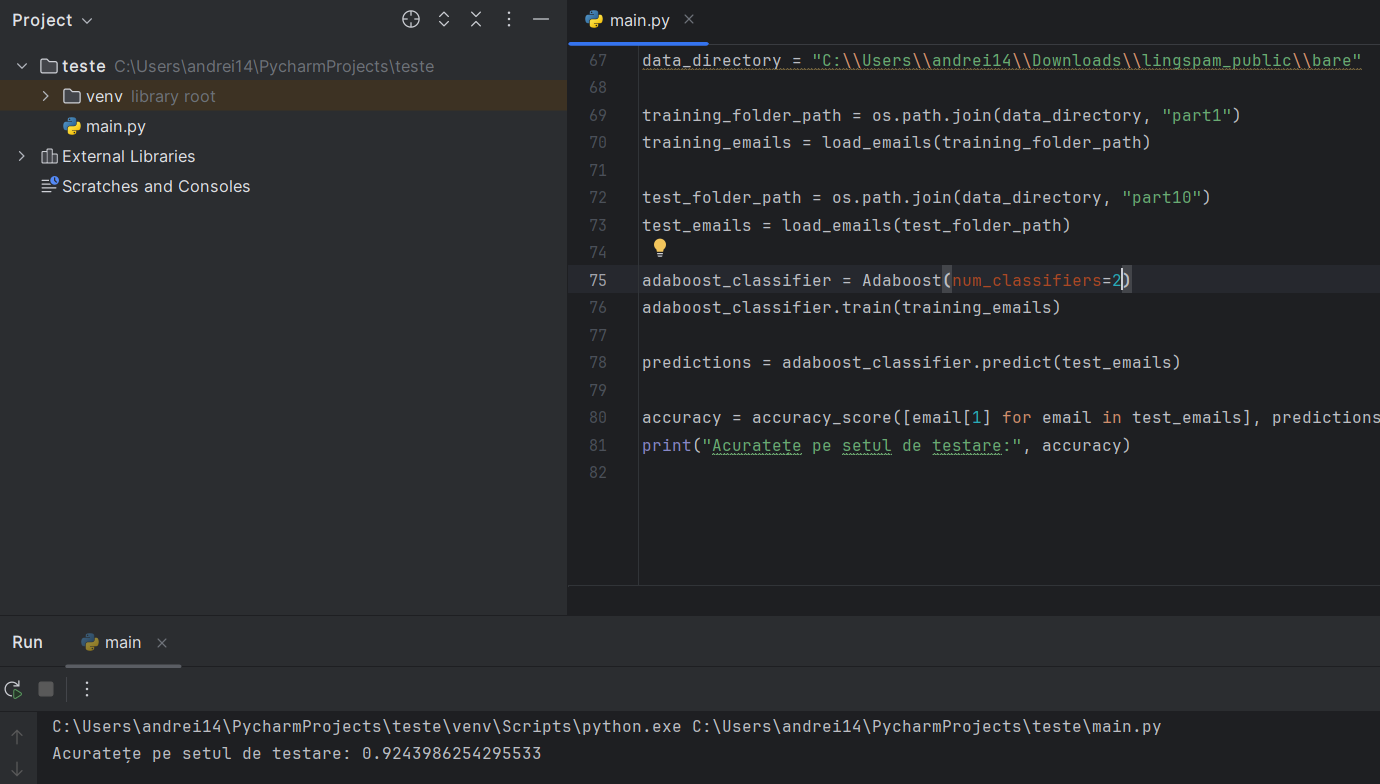
\includegraphics[scale=0.6]{adaboost2} \\\\
		Mai jos, acuratetea pentru algoritmul ID3, una de aproximativ 96.6\%, este cea care se apropie cel mai mult de cea obtinuta de Naive Bayes, dar are in continuare un procent care poate fi semnificativ sub Naive Bayes.\\\\
		\\\\\\\\\\\\\\\\\\\\\\\\\\
		ACURATETE ID3 IN FUNCTIE DE ADANCIMEA MAXIMA\\
		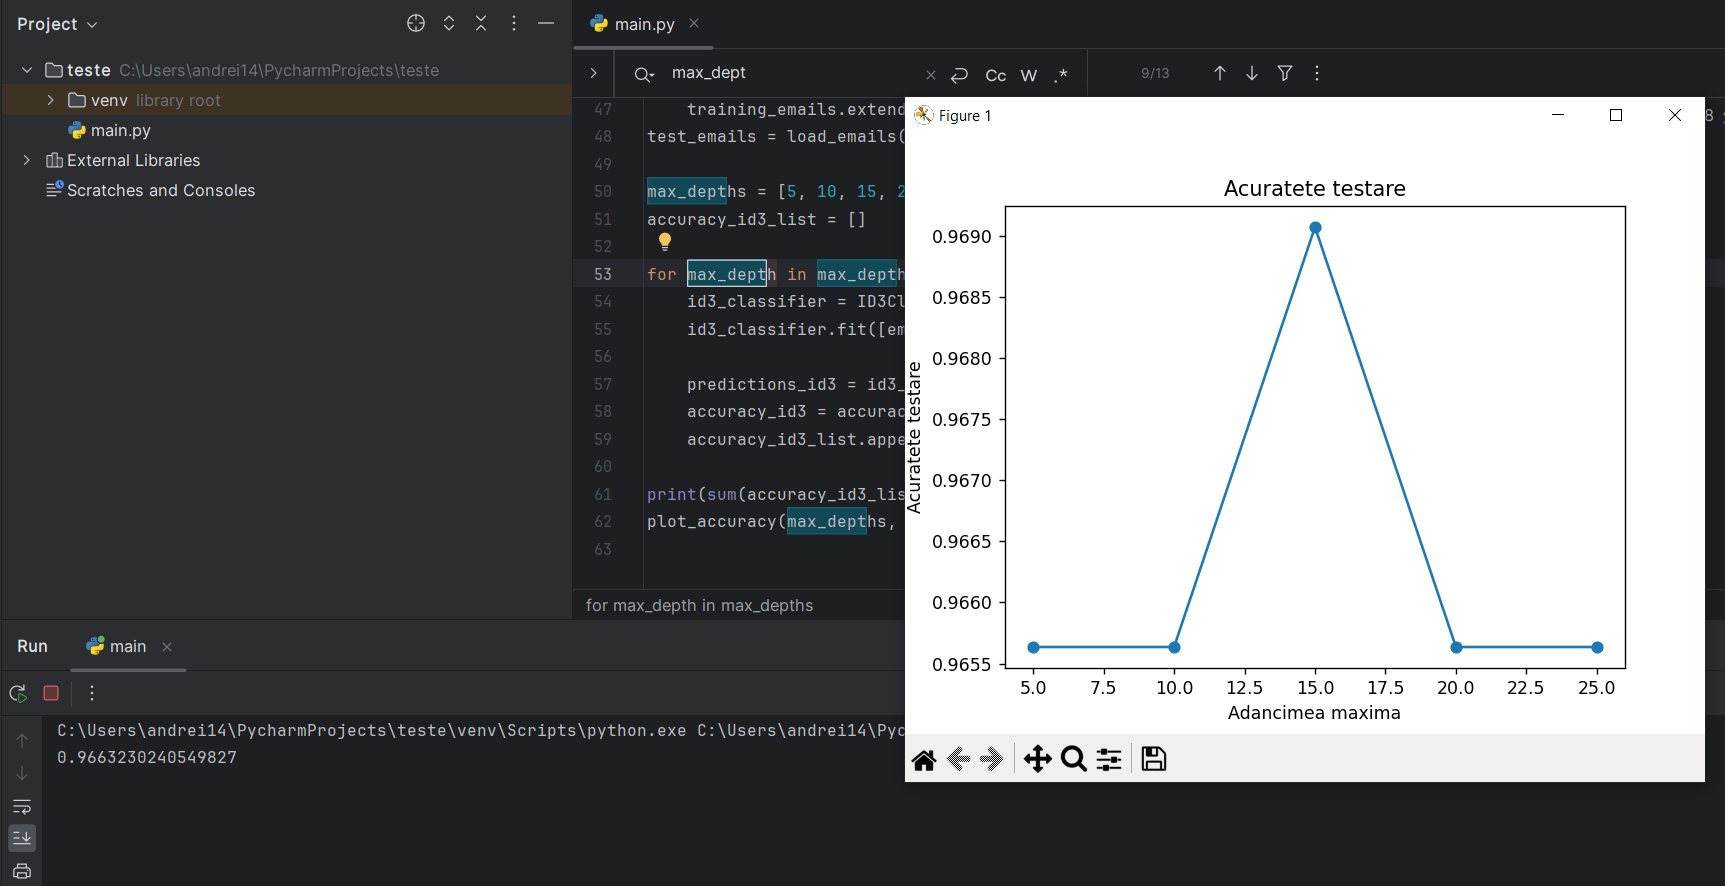
\includegraphics[scale=0.5]{id3}\\\\
		Cele 2 implementari pentru Adaboost si ID3 au fost implementari simple folosind notiunile deja existente din sklearn si nu implementari complete cum este cea pentru Naive Bayes.
		\\\\
		Pe baza rezultatelor practice, dar si a informatiilor teoretice, am observat ca Naive Bayes obtine o performanta superioara pentru acest tip de problema fata de ceilalti algoritmi studiati si este de asemenea si mai usor si mai intuitiv de implementat.
	}
\\\\
	{\large \underline{LOOCV} }
	\\\\
	{\normalsize 
		Dupa cum se poate observa mai jos, acuratetea LOOCV este aproximativ 97\%, aproximativ egala cu acuratetea pe setul de date de test. Acest lucru arata ca modelul implementat are o buna putere de generalizare pe date noi si de asemenea, lipseste overfitting-ul.\\
		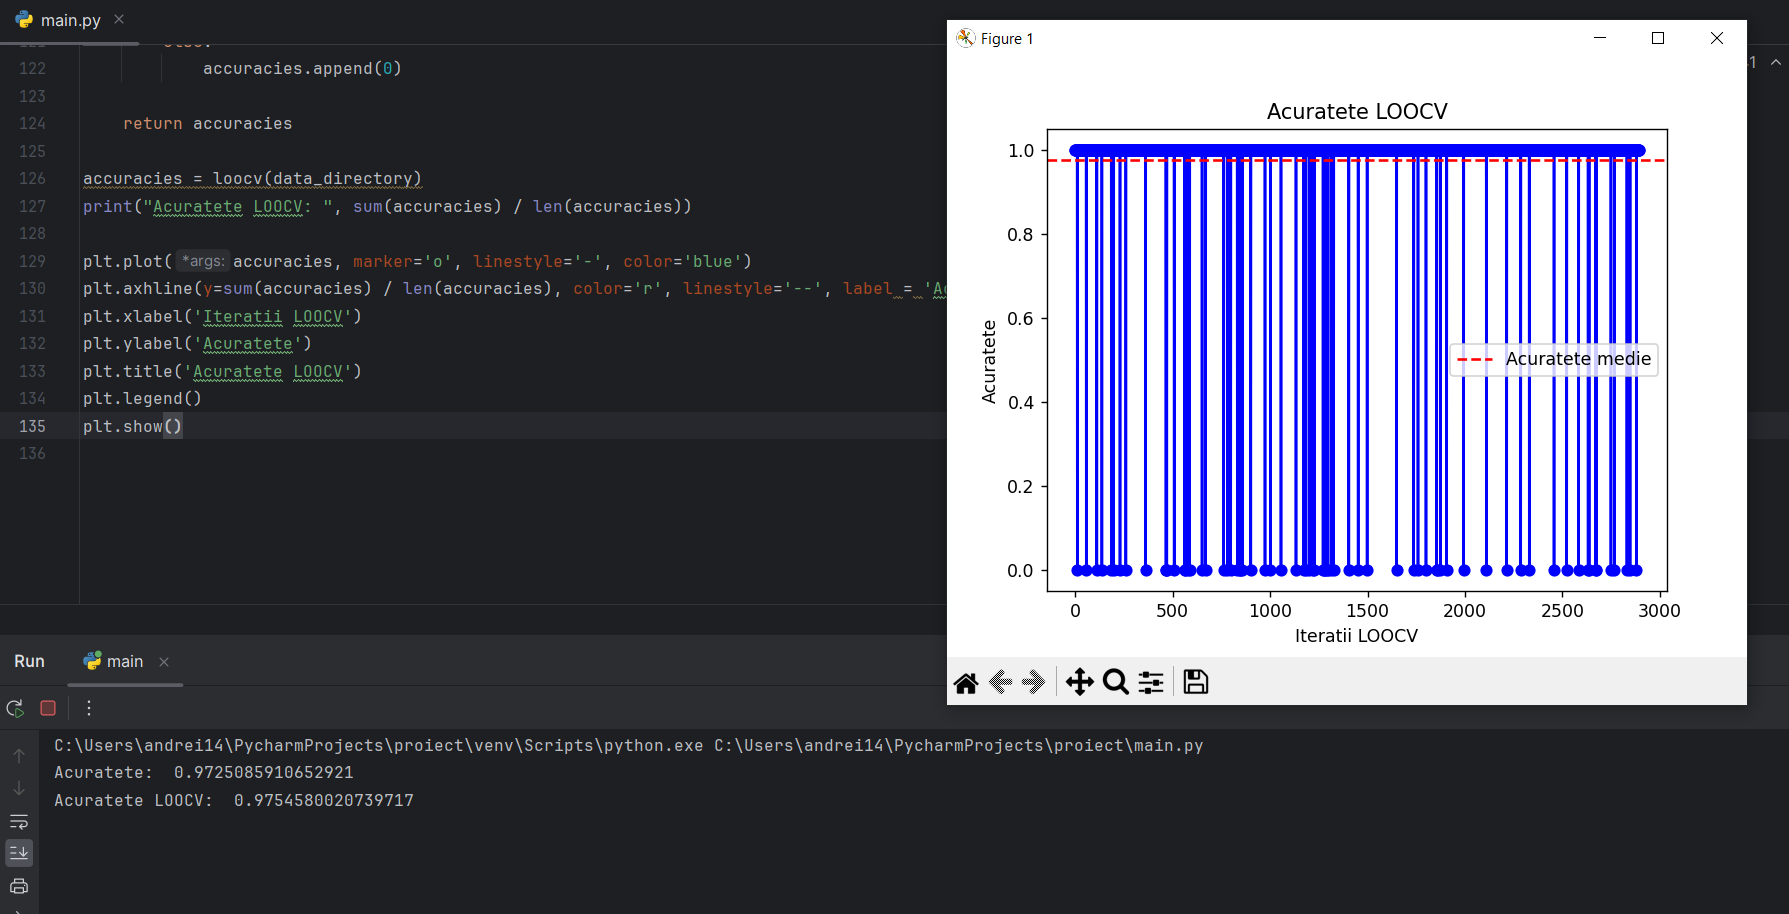
\includegraphics[scale=0.5]{acuratete}\\
		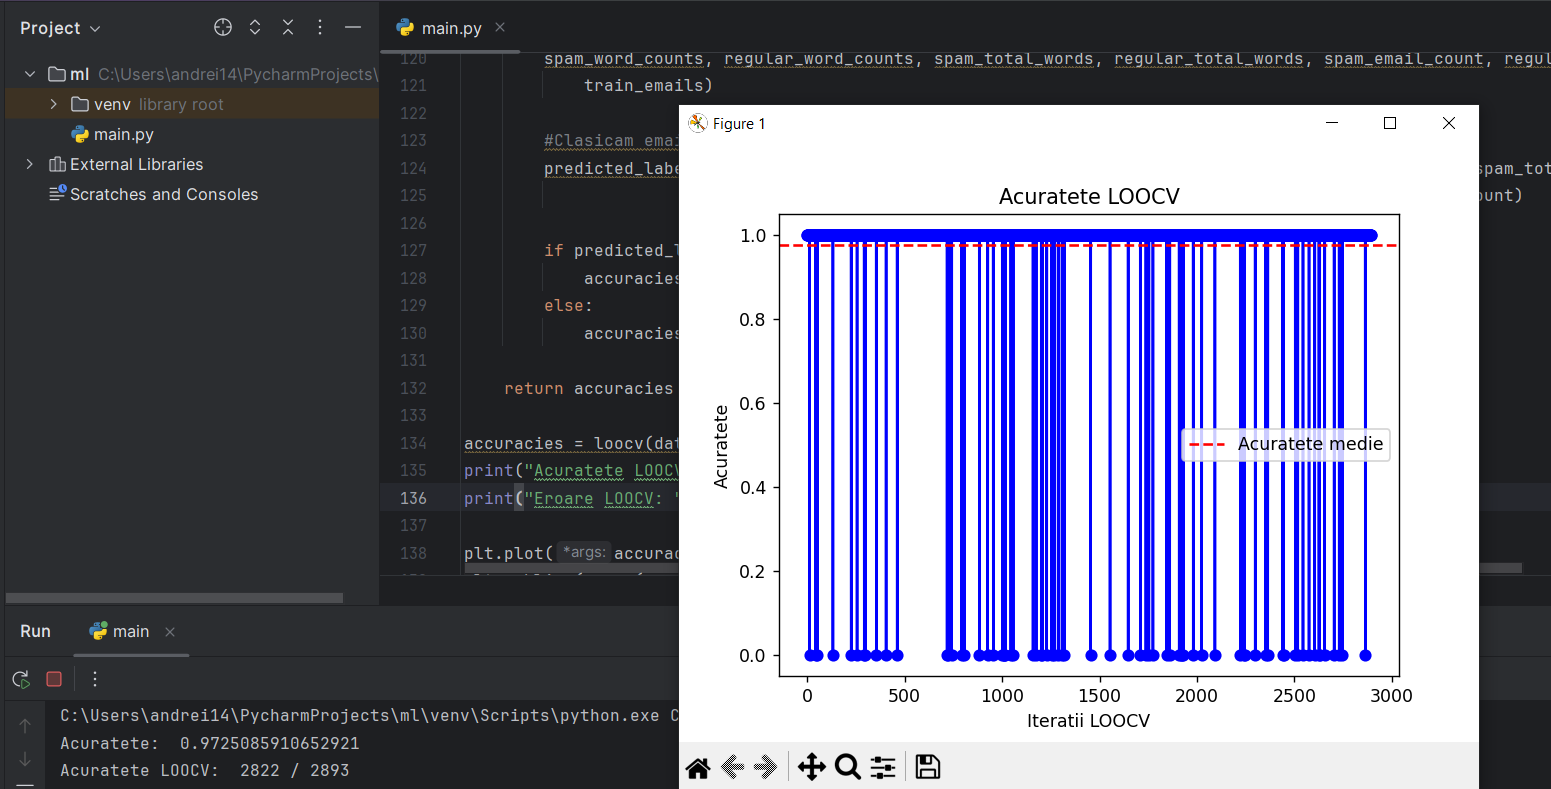
\includegraphics[scale=0.5]{acurateteloocv2}
	}
\end{document}